\chapter{Interfaz gráfica}
\label{cha:gui}

\section{Estructura}
Hasta ahora, las herramientas de verificación y minería mostradas en este proyecto utilizaban interfaces de usuario poco amigables para usuarios inexpertos: a través de línea de comandos para la herramienta STLEval, o mediante código fuente en Python para la biblioteca ParetoLib.

En este apartado proponemos un espacio donde el usuario tenga que simplemente adjuntar los ficheros de entrada con las señales y especificaciones, elegir la operación a realizar entre las opciones disponibles para finalmente visualizar y descargar los resultados en forma gráfica.

\begin{figure}[htb]
\centering
  \includegraphics[width=.95\linewidth]{images/uml_diagram}
\caption{Estructura del proyecto}
\label{fig:est}
\end{figure}

Tal y como vemos en la figura \ref{fig:est}, la nueva interfaz gráfica de usuario se comunica con la biblioteca de minería ParetoLib. ParetoLib nos permite evaluar propiedades con parámetros, utilizando en ese caso los métodos nativos de la biblioteca; o sin parámetros, redirigiendo la consulta a través de una adaptación de la interfaz anterior. A su vez, ParetoLib está conectado por el otro extremo a los binarios precompilados y la API de STLEval.

%La manera original de realizar las consultas a través de la terminal obligaba a hacerlas por separado a STLEval a la biblioteca de minería dependiendo si quisiésemos una consulta STL paramétrica o no.
Originariamente, el formato de las especificaciones en STL obligaba a interacturar con la herramienta STLEval o la biblioteca ParetoLib por separado según si las ecuaciones incluían parámetros o no (componente azul de la imagen).
La nueva interfaz gráfica de usuario unifica el proceso y facilita la usabilidad de cara al usuario.


Como aportaciones nuevas al proyecto (marcadas en rojo) está la propia interfaz gráfica de usuario, los operadores derivada e integral en STLEval y una modificación en la API paramétrica de STL, con la cual conseguimos ejecutar consultas no paramétricas desde ParetoLib.

\section{Bibliotecas utilizadas}

Debido a que la biblioteca ParetoLib está escrita en Python, y que con una pequeña modificación de la interfaz de interconexión permite acceder indirectamente a la API de STLEval, hemos decidido desarrollar la interfaz gráfica de usuario en ese mismo lenguaje. Para la elaboración de la parte gráfica de este proyecto hemos hecho uso de las bibliotecas:
\begin{itemize}
\item \href{https://www.qt.io/qt-for-python}{PyQt5}
\item Matplotlib
\item Pandas
\item Seaborn
\end{itemize}
 
\subsection{PyQt5}
La biblioteca PyQt5 está basada en la biblioteca gráfica Qt y sirve para realizar el diseño gráfico de la ventana principal de la aplicación desde Python. En nuestro caso optamos por un diseño simple de dos columnas: en la parte izquierda tenemos los botones y opciones para importar los ficheros de señales y la especificación de la operación, además de un espacio adicional para otras operaciones nuevas a implementar en un futuro. Al lado derecho tenemos la visualización de las señales tratadas y la especificación STL importada, la cual sólo se puede visualizar en modo lectura (es decir, los cambios en la especificación STL no se registrarán para la evaluación). Para extraer todo el potencial de PyQt5 hemos hecho uso de la herramienta \textit{Qt Designer}. Gracias a ella hemos podido construir el boceto de la interfaz, sobre la que después hemos anclado manualmente las funcionalidades a los botones correspondientes.

\begin{figure}[htb]
\centering
  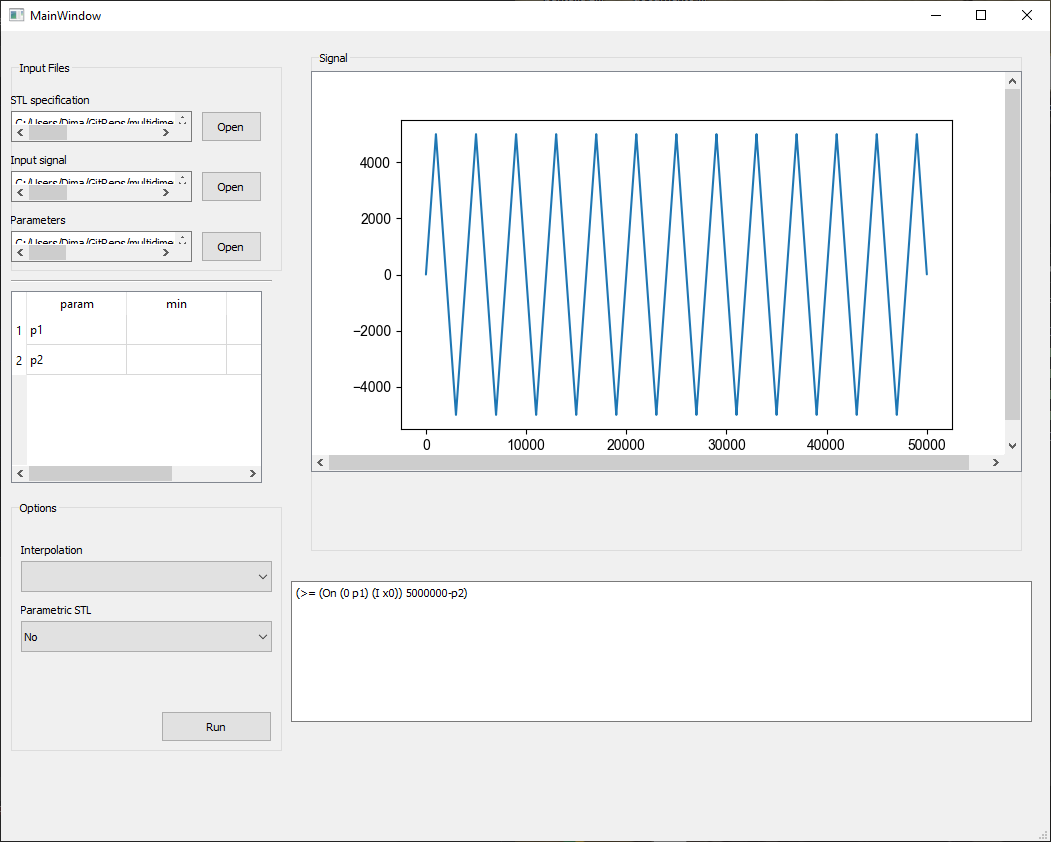
\includegraphics[width=1.0\linewidth]{images/gui} 
\caption{La ventana principal}
\label{fig:gui}
\end{figure}

%Instalación: 
%El desarrollo de la aplicación se hizo en un entorno linux haciendo uso del gestor de paquetes “pip”. 
 
%1 - Antes de todo, tenemos que confirmar la versión de Python que tenemos instalada con ´python3 --version´.
 
%2 - En el caso de que no lo tuviésemos, instalamos el gestor de paquetes “pip” con sudo ‘apt-get install python3-pip’ y actualizamos el mismo ´pip install -U pip´ 
 
%3 - Instalamos la librería PyQT con ´pip install pyqt5´. 
 
\subsection{MatplotLib}
La biblioteca MatplotLib da soporte a la mayoría de las bibliotecas gráficas avanzadas en Python (p.ej., Seaborn). Desde la versión inicial de ParetoLib, accesible únicamente a nivel de código fuente en Python, MatplotLib se utiliza para generar los gráficos resultantes de la minería de propiedades STL paramétricas (Figuras~\ref{fig:param_derivative}--\ref{fig:param_integral}). El uso del entorno PyQt5 para el diseño de la ventana principal de la nueva interfaz gráfica de usuario obliga a reajustar ligeramente la producción de estas imágenes de resultado para que se impriman dentro de una nueva ventana flotante en PyQt.
 
%Instalación: 
 
%1 - En este caso es sumamente simple realizando: ´sudo apt-get install python3-matplotlib´.
 
\subsection{Pandas}
La biblioteca Pandas es una biblioteca de Python especializada en el manejo y análisis de grandes bloques de datos. En nuestro caso, usamos esta biblioteca para la lectura lectura de las señales de entrada, las cuales están en ficheros csv y pueden albergar incluso miles de puntos.

Con esta biblioteca realizamos la transformación y almacenamiento de nuestras señales en una estructura de datos intermedia tipo \textit{DataFrame}, la cual utilizamos posteriormente como dato de entrada para los métodos de visualización gráfica de la señal a través de la biblioteca Seaborn.
 
%Instalación: 
 
%1 - Instalamos la librería con el comando: ´pip install pandas´

\subsection{Seaborn} 
Basada en MatplotLib, Seaborn es una biblioteca que permite generar fácilmente elegantes gráficos. Nosotros la utilizamos para dibujar las señales a partir de los datos importados en los archivos csv.

La función de esta biblioteca es meramente estética: creemos que este recurso es principalmente un añadido atractivo a la herramienta que puede ser útil en el caso que se quiera realizar presentaciones sobre sus resultados gráficos. Además, damos pie y esperamos poder realizar una mejora en todas las partes más visuales del aplicativo.
 
%Instalación: 
 
%1 - Instalamos la librería con el comando: ´pip install seaborn´

\section{Guía de uso}
En esta sección vamos a describir alguna de las partes interactuables o visibles de la interfaz gráfica de usuario:

\begin{itemize}
\item STL specification: Permite seleccionar un archivo \textbf{.stl}, el cual contiene una formula en STL (paramétrica o no). Cuando seleccionamos el archivo, la descripción de la formula aparece en una caja inferior en modo lectura (es decir, no modificable). Según si la consulta al motor de aprendizaje es paramétrica o no, habrá que modificar el casillero \textit{Parametric STL}.

\item Input signal: Permite seleccionar un archivo \textbf{.csv} que contiene la definición de la señal. Una vez seleccionado aparece un dibujo de esta en la caja grande de la ventana.

\item Parameters: Permite seleccionar un archivo \textbf{.param} que contiene los parámetros a estudiar y que aparecen en la formula del archivo .stl seleccionado. Es un fichero opcional: para una consulta no paramétrica no hace falta seleccionar ningún archivo. Al elegir un archivo, aparecerá más abajo una caja donde se deberá rellenar el intervalo de búsqueda (valores mínimo y máximo) de cada parámetro sobre los que la biblioteca de ParetoLib realizará el aprendizaje.

\item Parametric STL: Permite seleccionar si evaluaremos una consulta STL paramétrica o no: en el caso de quererla, seleccionamos que sí y viceversa.

\item Run: Permite ejecutar la consulta. Para poder hacerla necesitamos los tres ficheros de entrada anteriores descritos (dos ficheros en el caso no paramétrico). El clic de este botón recoge las rutas de los ficheros de entrada, el rango de valores numéricos de los parámetros (en el caso de haberlos) y prepara la invocación a la biblioteca de minería de forma similar al código mostrado en el código fuente \ref{list:paretolib_example}. En el caso de ser una consulta paramétrica, se nos devolverá un mapa con las regiones falsas o verdaderas según los parámetros (Figuras~\ref{fig:param_derivative}--\ref{fig:param_integral}). En el caso contrario, si la consulta no es paramétrica, simplemente devolverá el resultado de la evaluación: \textit{True} o \textit{False} (Figura~\ref{fig:noparam}).
%\textit{True} \ref{fig:noparam_true} o \textit{False} \ref{fig:noparam_false}.
\end{itemize}

%\begin{figure}[htb]
%\centering
%  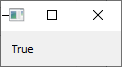
\includegraphics[width=0.3\linewidth]{images/stl_noparam_true} 
%\caption{Resultado no paramétrico True.}
%\label{fig:noparam_true}
%\end{figure}
%
%\begin{figure}[htb]
%\centering
%  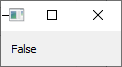
\includegraphics[width=0.3\linewidth]{images/stl_noparam_false} 
%\caption{Resultado no paramétrico False.}
%\label{fig:noparam_false}
%\end{figure}

\begin{figure}
\centering
  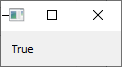
\includegraphics[width=0.3\linewidth]{images/stl_noparam_true} \hfill
  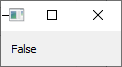
\includegraphics[width=0.3\linewidth]{images/stl_noparam_false} 
\caption{Resultado no paramétrico.}
\label{fig:noparam}
\end{figure}